\documentclass[11pt]{article}
\usepackage[margin=1in]{geometry}
\usepackage{fontspec}
\usepackage{amsmath}
\usepackage{booktabs}
\usepackage{array}
\usepackage{longtable}
\usepackage{graphicx}
\usepackage{float}
\usepackage[font=small,labelfont=bf]{caption}
\usepackage{natbib}
\usepackage{xurl}
\usepackage[hidelinks]{hyperref}
\usepackage{setspace}
\setstretch{1.15}
\renewcommand{\topfraction}{0.9}
\renewcommand{\textfraction}{0.1}
\renewcommand{\floatpagefraction}{0.75}
\newcommand{\nBootstrap}{5,000}
\newcommand{\nLooDraws}{2,000}
\newcommand{\analysisSeed}{20261009}
\newcommand{\nCohort}{359}
\newcommand{\nEligible}{293}
\newcommand{\nExcludedPosition}{66}
\newcommand{\nPaired}{291}
\newcommand{\nSupport}{159}
\newcommand{\nOppose}{132}
\newcommand{\nOmitted}{2}
\newcommand{\corePreC}{82.5}
\newcommand{\corePostC}{87.9}
\newcommand{\corePreU}{58.1}
\newcommand{\corePostU}{76.0}
\newcommand{\coreGainC}{5.4}
\newcommand{\coreGainU}{18.0}
\newcommand{\coreDiff}{12.6}
\newcommand{\coreLow}{3.8}
\newcommand{\coreHigh}{21.4}
\newcommand{\coreComposition}{11.7}
\newcommand{\arrivalDiff}{8.8}
\newcommand{\arrivalLow}{0.8}
\newcommand{\arrivalHigh}{17.0}
\newcommand{\arrivalN}{286}
\newcommand{\substantiveDiff}{15.1}
\newcommand{\substantiveLow}{5.9}
\newcommand{\substantiveHigh}{24.4}
\newcommand{\substantiveN}{221}
\newcommand{\pilotDiff}{8.4}
\newcommand{\withoutBankDiff}{13.8}
\newcommand{\nPilotItems}{23}
\newcommand{\nPilotAgree}{19}
\newcommand{\pilotAgreement}{82.6}
\newcommand{\pilotKappa}{0.768}
\newcommand{\nPilotPeople}{4,475}
\newcommand{\nPilotRows}{32,043}
\newcommand{\nDuplicates}{93}
\newcommand{\coreHeadroom}{18.9}

\newcommand{\inventoryItems}{260}
\newcommand{\inventoryStudies}{32}
\newcommand{\codedStudies}{16}
\newcommand{\primaryStudies}{14}
\newcommand{\primaryItems}{28}
\newcommand{\comparativePeople}{4400}
\newcommand{\positiveGainStudies}{13}
\newcommand{\positiveDifferenceStudies}{11}
\newcommand{\positiveIntervalStudies}{2}
\newcommand{\comparativeDraws}{5,000}
\newcommand{\comparativeMin}{-7.3}
\newcommand{\comparativeMax}{15.6}
\newcommand{\niGainC}{42.0}
\newcommand{\niGainU}{35.2}
\newcommand{\niDifference}{-6.9}
\newcommand{\niLow}{-19.2}
\newcommand{\niHigh}{8.1}
\newcommand{\usGainC}{12.4}
\newcommand{\usGainU}{14.6}
\newcommand{\acaPolicyDiff}{1.9}
\newcommand{\acaPolicyLow}{-9.4}
\newcommand{\acaPolicyHigh}{13.6}
\newcommand{\sanMateoN}{83}
\newcommand{\sanMateoCanonicalN}{165}
\newcommand{\sanMateoDiff}{2.2}
\newcommand{\sanMateoCanonicalDiff}{-5.4}
\newcommand{\partyGainC}{2.8}
\newcommand{\partyGainU}{2.4}
\newcommand{\partyDifference}{-0.4}
\newcommand{\partyLow}{-12.1}
\newcommand{\partyHigh}{11.7}

\newcommand{\tabnote}[1]{\par\smallskip\begin{minipage}{\linewidth}\footnotesize #1\end{minipage}}
\title{The Awful Truth:\\Learning Facts That Favor the Other Side}
\author{}
\date{Working draft, October 2026}

\begin{document}
\maketitle
\begin{abstract}
\noindent Equally knowledgeable people on opposite sides of a dispute may know different things. Does deliberation help them learn facts that favor the other side? We classify factual questions by their implications for respondents' pre-event positions and compare paired changes in accuracy on the same questions. A systematic screen of \inventoryItems{} items across \inventoryStudies{} studies yields a primary comparison covering \primaryItems{} items in \primaryStudies{} Deliberative Polls. Uncongenial accuracy increases in \positiveGainStudies{} studies, but greater uncongenial than congenial gains are not uniform: the estimated difference is positive in \positiveDifferenceStudies{} studies, and only \positiveIntervalStudies{} conditional intervals exclude zero on the positive side. Northern Ireland shows substantial gains in both categories; a separate US party-alignment comparison is close to zero. The contribution extends Hansen's Danish selective-learning analysis into a comparative respondent-by-item design. The evidence supports learning across initial positions, with uneven relative catch-up. It does not identify a causal effect of deliberation or distinguish motivated learning from differences in initial knowledge, response behavior, and room to improve.
\end{abstract}

\section{Introduction}

Equally knowledgeable people on opposite sides of a policy dispute may know and not know different things. One may know a policy's costs, another its benefits. Their total knowledge scores can be identical while the considerations available to them differ. Deliberation asks people to confront facts and arguments they might otherwise overlook. Whether they learn facts that favor the other side is therefore a different question from whether their overall knowledge increases.

Across the studies examined here, people generally become more accurate on facts that challenge their initial positions. But those gains do not consistently exceed gains on congenial facts. The primary comparison covers \primaryStudies{} studies, including disputes about constitutional change, criminal justice, schools, foreign policy, housing, health care, and voting rules. Uncongenial gains are positive in \positiveGainStudies{} studies. Relative catch-up is less uniform, and most study-specific contrasts remain imprecise. The Danish euro poll supplies a clear example of catch-up; it does not describe every setting.

Selective learning in Denmark is already the subject of \citet[sec.~6.5, Table~6.8]{hansen2004}. Hansen divided respondents by recruitment voting intentions, interpreted particular euro facts, and showed that several initial knowledge gaps narrowed. The broader analysis of that event also examined knowledge and opinion change \citep{andersen2007}. Neither the question nor the Danish pattern is a new discovery. Our contribution is the comparative construction: an explicit respondent-by-item relation, a systematic screen of the retained questions, matched pre-event positions, and a common comparison that can accommodate studies whose factual batteries favor only one side of an issue.

The relation between a person and a fact must be established independently of the person's answer. Political knowledge gaps vary across subjects, and apparent differences can depend on wording and response behavior \citep{jerit2012,roush2023}. A question that one side answers less accurately is not thereby uncongenial to that side. Defining uncongeniality by an initial knowledge deficit would also build room for catch-up into the outcome. We instead combine the substantive implication of the correct proposition with a position or group affiliation measured before the event.

\section{Facts, Groups, and Positions}

A fact is congenial here when its policy implication supports a respondent's baseline position, and uncongenial when it challenges that position. Congeniality is a relation, not an intrinsic property of a question. The same proposition can support one person's position and challenge another's. The classification does not assert that either person likes the fact, regards it as decisive, or consciously processes its political implications. Those are additional psychological claims.

Facts can bear on a policy without proving which policy is best. An uninsured population's low income is relevant to an argument for financial assistance; it does not settle how assistance should be financed. A requirement to offer a broad school curriculum can support sharing courses across schools; it does not prove that sharing outweighs every objection. Requiring a fact to logically determine the whole policy choice would eliminate much of the information that citizens actually use in political argument.

Group membership supplies a different reference point. A fact can challenge a party's stated position even when an individual party member disagrees with that position. We therefore distinguish personal policy congeniality from documented party alignment. A further distinction concerns knowledge \emph{about} another group. Knowing a minority's population share or living conditions is outgroup knowledge for some respondents, but its substantive implication need not favor that group. Research on deliberative contact includes such factual knowledge \citep{kim2018}; it cannot be merged automatically with position-relative congeniality.

Learning also need not produce agreement. People may accept a fact yet disagree about its importance or consequences \citep{gaines2007}. Changes in correct-answer scores can reflect recall, guessing, or willingness to report an answer already known. Accuracy incentives in factual-learning studies show why motivated responding and motivated learning should remain distinct \citep{khanna2018}. We use learning as shorthand for increased reported factual accuracy, without treating a score change as a uniquely identified psychological process.

The comparative design separates two descriptive propositions. Broadening requires positive gains on uncongenial facts. Relative catch-up requires those gains to exceed congenial gains. The latter is a stronger statement about scores, but not necessarily stronger evidence of a change in motivation. When congenial accuracy starts higher, an identical acquisition process can produce a larger uncongenial increase simply because more errors remain to be corrected.

\section{Data and Research Design}

Deliberative Polls combine a recruited public sample with opportunities to consider competing information and discuss public choices \citep{fishkin2005}. The unit of analysis is a respondent answering a particular factual question before and after a Deliberative Poll. We begin with the complete retained item inventory, rather than selecting events from their learning results. The archive contains \inventoryItems{} questions in \inventoryStudies{} studies. Historical writing in the project supplies the comparative question; archived questionnaires, briefing materials, answer keys, and respondent files supply the measurement. We use one respondent namespace per study and retain verified attendees. Recruitment measurements precede the event; the second measurement is the immediate post-deliberation questionnaire. These windows can include briefing exposure and repeated testing as well as discussion.

\subsection{Coding the relationship between a person and a fact}

Each item receives a correct proposition, an explicit policy axis, a direction on that axis, and a source-based rationale. A direction requires a recognizable argument, benefit, cost, or objection. It does not require the fact to settle the entire policy dispute. The baseline questionnaire then locates the respondent on that same axis. A fact supporting the respondent's position is congenial; one challenging it is uncongenial. Undecided respondents, scale midpoints, missing answers, and unresolved item meanings remain \emph{cannot classify}. They are excluded from the directional contrast, but their records and reasons are retained. An analyst's inability to classify a relation differs from a respondent's don't-know answer to a classified question.

For example, the US health-care item asks about protections provided by the Affordable Care Act. Those protections supply an argument for retaining the law. The baseline item asks whether to repeal it, so its response scale is reversed for a retention axis. In Northern Ireland, the curriculum entitlement supplies a reason for sharing courses across schools. We use baseline support for pupils taking unavailable courses at another school, not religious identity, to locate respondents on that policy axis. In Australia, we use support for the particular referendum proposal, not generic enthusiasm for a republic.

Group alignment is a separate classification. For the US health-care item, the archived Democratic and Republican platforms document opposing positions on retaining the law \citep{democrats2016,republicans2016}. We therefore report an additional comparison defined by baseline party identification. Independents and respondents without a major-party identification remain unclassified for that comparison. This coding concerns a fact's implications for a party's stated position; it does not claim that every member personally holds that position. We do not infer an analogous Catholic--Protestant policy division from religious identity alone.

Two independent model-assisted passes screened the full inventory. Their records preserve rationale, source locators, uncertainty, and disagreements. An initial adjudication fixed a primary mapping and a broader sensitivity mapping before inspection of the new comparative outcomes. A subsequent source audit moved a flawed Vermont item out of the primary set; the appendix documents that retrospective correction. The primary mapping uses the clearest source-supported arguments and matched baseline questions; the expanded mapping admits additional interpretation-dependent arguments. Agreement between model passes is not human validation. Moreover, this is retrospective work: the earlier Danish analysis was already known, and some codebook searches exposed aggregate item summaries. No initial subgroup knowledge gap or observed learning contrast determines an item's direction. The coding records disclose these exposures, and all intervals condition on the chosen mapping.

\subsection{Comparing learning on the same facts}

Let $Y_{ijt}$ indicate a correct answer by respondent $i$ to item $j$ at time $t$, and let $R_{ij}$ denote the relation fixed from baseline. For each item and relation $r$, we retain respondents with both pre- and post-event scores and estimate
\[
\widehat\Delta_{jr}
=\frac{1}{n_{jr}}\sum_{i:R_{ij}=r}
  (Y_{ij,\mathrm{post}}-Y_{ij,\mathrm{pre}}).
\]
The study-level gain is the equal-weighted mean over the same set $J$ of items with observed congenial and uncongenial respondents:
\[
\widehat L_r=\frac{1}{|J|}\sum_{j\in J}\widehat\Delta_{jr},
\qquad
\widehat D=\widehat L_U-\widehat L_C.
\]
Levels use the same paired respondents within each item. Equal item weights prevent a difference in question composition from defining the congenial--uncongenial comparison. They do not remove differences between the respondents on each side.

Pairing here refers to the same respondent answering the same question at two times. It does not generally mean that the same person contributes to both relation categories. A battery containing only facts favoring school collaboration still permits a comparison between initial supporters and opponents. Discarding such a battery would unnecessarily restrict the comparative inquiry. Its limitation is substantive: relation and baseline group may be completely aligned, so a difference in gains can reflect any difference between those groups. The Danish complete-battery, equally weighted supporter--opponent analysis remains a separate within-person sensitivity analysis.

We report study-specific estimates rather than treating the studies as a random sample of political disputes. Recruitment, topics, instruments, modes, and event formats differ. Each study receives its own uncertainty interval; we do not interpret the number of positive estimates as a formal test across independent replications. Explicit don't-knows receive zero credit. Undocumented source blanks and absent waves are missing. Sensitivity analyses use the archive's canonical scoring and, separately, substantive responses only. The latter conditions on willingness to answer and can change the sample.

Bootstrap intervals resample complete discussion groups where group identifiers are available for the analytic sample; otherwise they resample respondents and leave discussion dependence unaddressed. All of a resampled respondent's item pairs travel together. We use \comparativeDraws{} draws and percentile 95\% intervals, holding the eligible item set fixed within a specification. The outputs report sparse cells and draws that lack a required item--relation cell. The estimator suppresses intervals for singleton resampling-unit cells or inadequate valid draws. Following the support audit, the manuscript also withholds intervals with fewer than five units in any included relation cell or partially missing discussion-group identifiers. Intervals from few groups warrant particular caution; none incorporates uncertainty in substantive coding.

\subsection{What the comparison identifies}

A positive $L_U$ establishes increased reported accuracy on facts coded as uncongenial. A positive $D$ establishes relative catch-up. Neither identifies a causal effect of deliberation: attendees are selected, exposure is bundled, the comparison groups are not randomized to congeniality, and testing itself may change answers. Nor does relative catch-up establish a special willingness to learn uncomfortable facts.

Initial accuracy matters because a binary score leaves unequal room for improvement. If the probability of correcting a wrong answer is $a$ and the probability of losing a correct answer is $\ell$, an item with initial accuracy $p$ has expected gain $a(1-p)-\ell p$. With the same transition probabilities in both categories, the uncongenial-minus-congenial difference is $(a+\ell)(p_C-p_U)$. Thus an initial congenial advantage alone can produce faster uncongenial gains. We report baseline levels alongside changes and use the earlier Danish transition calculation as a diagnostic, not as an identified account of the mechanism.


\section{Results}

\subsection{Learning across initial positions}

Uncongenial accuracy increases in \positiveGainStudies{} of the \primaryStudies{} primary studies (Table~\ref{tab:comparative}). The studies differ greatly in the size of those gains. The pattern establishes that respondents often become more accurate on information supporting a position they initially opposed. It does not require an initial knowledge disadvantage, nor does it imply that the information changes their policy preferences.

\begin{table}[!htbp]
\centering\scriptsize
\setlength{\tabcolsep}{3.5pt}
\caption{Paired changes on the same facts across baseline policy positions.}
\label{tab:comparative}
\begin{tabular}{lrrrrrl}
\toprule
Study & Items & People & C gain & U gain & U--C & 95\% interval \\
\midrule
Britain: crime (1994) & 2 & 261 & 29.4 & 34.0 & 4.6 & [-16.6, 29.2] \\
Britain: health (1998) & 1 & 165 & 3.7 & 0.0 & -3.7 & -- \\
Australia: republic (1999) & 2 & 300 & 51.4 & 54.3 & 2.9 & [-5.8, 11.0] \\
Denmark: euro (2000) & 2 & 293 & 5.3 & 18.0 & 12.7 & [3.8, 21.6] \\
Bulgaria: crime (2002) & 1 & 232 & -1.9 & 5.1 & 7.1 & [-6.0, 19.0] \\
US: online foreign policy (2003) & 2 & 205 & 7.5 & 12.6 & 5.1 & [-11.4, 22.2] \\
US: foreign policy (2003) & 2 & 285 & 20.9 & 21.5 & 0.6 & [-11.8, 12.6] \\
US: election (2004) & 3 & 215 & 9.2 & 12.5 & 3.3 & [-4.9, 11.5] \\
US: health/education (2005) & 2 & 385 & 11.2 & 3.9 & -7.3 & [-14.1, 0.3] \\
US: citizenship (2007) & 2 & 288 & 2.6 & 18.2 & 15.6 & [3.7, 27.4] \\
Northern Ireland: schools (2007) & 3 & 117 & 42.0 & 35.2 & -6.9 & [-19.2, 8.1] \\
San Mateo: housing (2008) & 3 & 83 & 10.4 & 12.6 & 2.2 & [-22.2, 24.9] \\
US: America in One Room (2019) & 2 & 485 & 12.4 & 14.6 & 2.2 & [-6.2, 10.7] \\
Multinational: antibiotics (2024) & 1 & 1086 & 11.5 & 18.2 & 6.7 & [-13.2, 27.7] \\
\bottomrule
\end{tabular}

\tabnote{C denotes congenial and U uncongenial. Gains and U--C differences are percentage points, averaged equally over the same items within each study. People counts are distinct respondents contributing at least one classifiable item pair; they need not contribute to both categories. The primary rule includes explicit don't-knows as incorrect and excludes undocumented source blanks. Intervals are conditional 95\% percentile bootstrap intervals, resampling discussion groups when complete identifiers are available and respondents otherwise. Intervals are omitted when any item--relation cell has fewer than five resampling units. The appendix reports baseline levels, cell support, and sensitivities.}
\end{table}

Northern Ireland makes the distinction between broadening and relative catch-up especially clear. The Omagh event brought Catholics and Protestants together to discuss the future of local schools \citep{luskin2014}. On the primary school-collaboration items, congenial accuracy rises by \niGainC{} points and uncongenial accuracy by \niGainU{} points. Both sides learn substantially. The difference is \niDifference{} points, with an interval from \niLow{} to \niHigh{}. The result offers no clear evidence of faster uncongenial learning, despite the large uncongenial gain. These relations use baseline preferences about shared campuses and shared courses, not an assumption that Catholics and Protestants favor opposing schooling policies.

The US America in One Room comparison similarly shows gains in both categories. Across the health-care and capital-gains items, congenial accuracy increases by \usGainC{} points and uncongenial accuracy by \usGainU{} points. Respondents are classified separately on each relevant policy question. Someone can therefore contribute a congenial health-care response and an uncongenial tax response, while another person contributes only one eligible pair. The item-balanced comparison accommodates those patterns without substituting party identity for the measured issue position.

\subsection{Relative catch-up is uneven}

The uncongenial-minus-congenial difference is positive in \positiveDifferenceStudies{} studies, but its magnitude ranges from \comparativeMin{} to \comparativeMax{} points (Figure~\ref{fig:comparative}). Only \positiveIntervalStudies{} of the conditional intervals exclude zero on the positive side. This count describes the displayed estimates; it is not a multiple-testing-adjusted conclusion or an estimate of how frequently deliberation produces catch-up in a population of events.

\begin{figure}[!htbp]
\centering
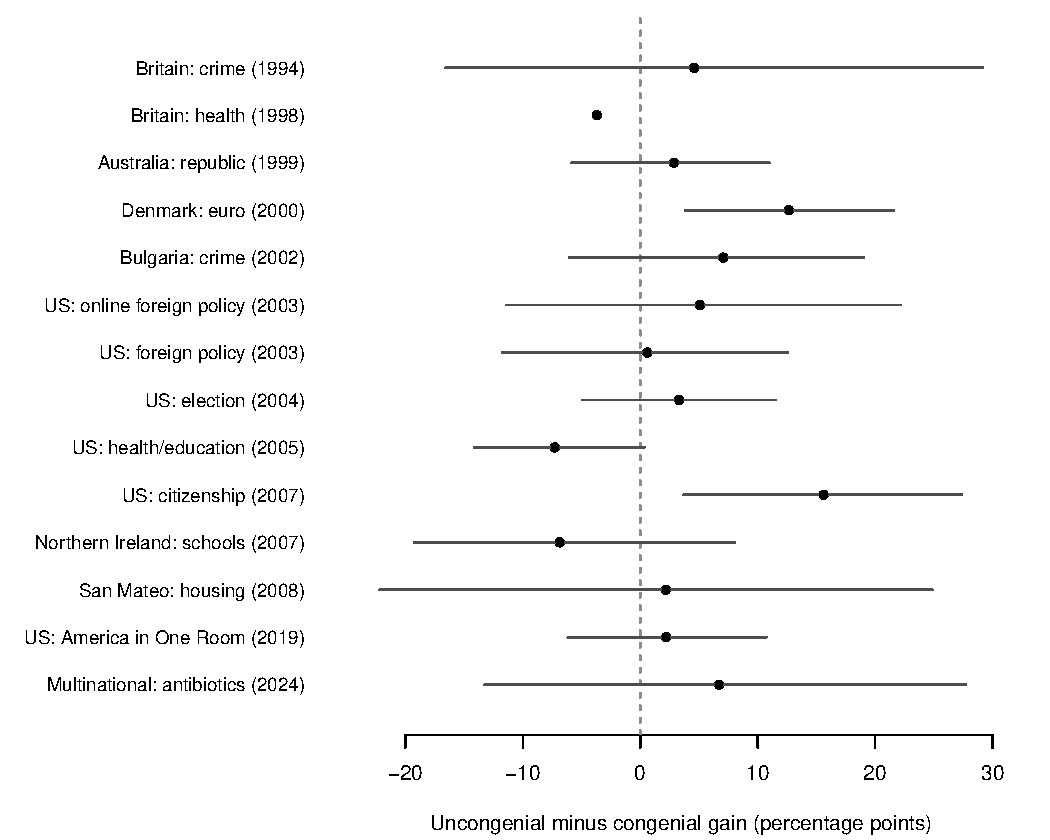
\includegraphics[width=\linewidth]{../figs/comparative_gains.pdf}
\caption{Relative catch-up varies across studies. Points show equal-item differences in paired accuracy gains, uncongenial minus congenial, for the primary policy-position comparison. Lines are conditional 95\% bootstrap intervals; resampling units and exclusions match Table~\ref{tab:comparative}. A positive value means larger uncongenial gains. Britain health has too few uncongenial resampling units for a displayed interval.}
\label{fig:comparative}
\end{figure}

The initial knowledge advantage is also uneven (Appendix Table~\ref{tab:comparative-levels}). Congenial accuracy often starts higher, but that ordering is weak or reversed in some studies. Denmark has a substantial initial asymmetry; Northern Ireland begins with nearly equal category accuracy. A universal account in which deliberation preferentially corrects uncomfortable errors would have to explain both the positive and negative differences. These data support a more limited conclusion: learning extends across initial positions, while its relative distribution depends on the topic, battery, and respondents.

Some apparently precise point estimates rest on very little opposing-position support. Britain health contains only a few uncongenial respondents under the selected baseline question. Its observed zero uncongenial gain is a finite-sample description, not evidence that opponents cannot learn. We retain the point estimate to show the coverage problem and omit its inferential interval. Item-by-relation counts remain available in the generated data.

\subsection{Party alignment and specification choices}

Neither version of the US health-care comparison shows clear relative catch-up. Democrats gain \partyGainC{} points on the ACA-protection item, while Republicans gain \partyGainU{} points. Under the documented platform mapping, the uncongenial-minus-congenial difference is \partyDifference{} points, with an interval from \partyLow{} to \partyHigh{}. On the same ACA item, classification by personal repeal preference yields a difference of \acaPolicyDiff{} points (\acaPolicyLow{} to \acaPolicyHigh{}). Both contrasts are imprecise and compatible with zero. They use different eligible groups, so their numerical difference does not identify an effect of party identification. The comparison keeps group alignment distinct from personal policy preference.

The broader item mapping does not restore a uniform catch-up pattern (Appendix Table~\ref{tab:comparative-sensitivity}). Adding interpretation-dependent facts changes some signs, including Northern Ireland and Australia. Different response rules also matter: excluding don't-knows selects a different set of answers, and treating source blanks as incorrect can change the observed sample as well as its scores. Those differences are part of the measurement result. A conclusion that depends on one plausible item mapping or missingness convention should remain conditional on it.

Denmark remains informative as a case with reciprocal item coverage and prior published analysis. The earlier complete-battery comparison gives an uncongenial-minus-congenial difference of \coreDiff{} points, with a conditional interval from \coreLow{} to \coreHigh{}. Broader Danish mappings preserve positive recruitment-to-exit contrasts. That result reproduces the substantive direction of Hansen's analysis while making the weighting and paired sample explicit. The cross-study variation limits how far the Danish pattern can be generalized.

\section{Discussion}

Deliberative participants often learn facts that favor positions they did not initially hold. That finding is broader than the Danish euro case. Faster learning of those facts is less general: both the estimated differences and their uncertainty vary across studies, and the separate party-defined comparison provides no clear evidence of relative catch-up. Aggregate knowledge gains alone would conceal these distinctions.

The main contribution is an explicit comparative measurement design. It connects an item's substantive implication to a pre-event respondent measure, retains uncertain relations, and compares changes on the same facts. It also permits useful evidence from one-direction batteries. Requiring each person to face both kinds of fact would discard much of the archive; retaining those studies requires acknowledging that the comparison is then between baseline groups.

The design leaves several questions open. Paired accuracy changes cannot isolate discussion from briefing, testing, or selection into attendance. Differences in gains cannot isolate congeniality from prior familiarity, education, political engagement, or group composition. Binary scores also impose unequal room to improve. Human adjudication of the model-assisted coding and new studies with balanced factual batteries would strengthen the measurement claim. A design that randomized exposure to equally difficult, independently coded congenial and uncongenial information would address a different and more causal question.

The original comparative ambition also includes learning about social outgroups. The present archive supports a distinction between policy and party alignment, but not a completed Roma versus non-Roma analysis of the Bulgarian Roma-policy event. The retained Bulgarian crime study cannot substitute for that event, and Northern Ireland's religious identities cannot substitute for measured schooling positions. Extending those comparisons requires linked group membership and clearly identified group-referent facts. The coding preserves those unresolved cases rather than converting them into null findings.

\clearpage
\bibliographystyle{apalike}
\bibliography{references}
\clearpage
\appendix
\section{Coverage and Measurement}

The inventory contains \inventoryItems{} retained factual questions from \inventoryStudies{} studies. Both expanded coding passes cover every item. Table~\ref{tab:coverage} distinguishes the inventory from the adjudicated analysis sets. A zero means that the current source review has not established an eligible directional mapping; it does not mean that respondents learned nothing or that no useful measure could ever be recovered. The complete machine-readable registry retains both coders' judgments and reasons, including neutral, ambiguous, and unresolved items.

Several exclusions concern measurement rather than data volume. Utility questionnaires often ask how important an energy objective is. Low importance does not identify opposition to that objective, so those scales do not supply the negative position needed here. Named-party placement questions can measure knowledge of what parties favor without establishing a fact favorable to those policies. Some studies have promising directional content but no sufficiently matched baseline field in the current adjudication. These remain explicit unresolved leads, rather than disappearing from the inventory.

The Bulgarian crime poll supplies a legal-constraint item about police violence. It is a different event from the Bulgarian poll concerning Roma policy. Reports and briefing materials for the latter exist, but linked respondent-level records have not been established in the retained archive. No Roma comparison is estimated. In Northern Ireland, religious affiliation is available, but neither community membership alone nor a fact about mixed schools establishes a unique policy implication for that community. The main analysis uses the relevant schooling preferences. The separate project on knowledge of arguments concerns a different outcome and is not counted as additional factual-knowledge evidence.

{\small\setstretch{1.0}
\begin{longtable}{lrrr}
\caption{Full retained inventory and adjudicated coverage.}\label{tab:coverage}\\
\toprule Study identifier & Inventory & Primary & Expanded total \\
\midrule\endfirsthead
\toprule Study identifier & Inventory & Primary & Expanded total \\
\midrule\endhead
a1r-climate-2021 & 8 & 0 & 0 \\
america-in-one-room-2019 & 7 & 2 & 2 \\
amr-2024 & 6 & 1 & 2 \\
australia-republic-1999 & 12 & 2 & 6 \\
btp-2007 & 8 & 2 & 3 \\
btp-general-election-2004 & 9 & 3 & 4 \\
btp-health-education-2005 & 6 & 2 & 3 \\
btp-national-2003 & 11 & 2 & 3 \\
btp-online-primaries-2004 & 7 & 0 & 0 \\
btp-presidential-primaries-2004 & 7 & 0 & 0 \\
bulgaria-crime-2002 & 7 & 1 & 1 \\
california-whats-next-2011 & 8 & 0 & 0 \\
cpl-1996 & 7 & 0 & 0 \\
denmark-euro-2000 & 9 & 2 & 4 \\
europolis-2009 & 9 & 0 & 0 \\
marousi-2006 & 7 & 0 & 0 \\
michigan-2009 & 11 & 0 & 0 \\
new-haven-2004 & 8 & 0 & 0 \\
nic-1996 & 11 & 0 & 0 \\
nic2-2003 & 11 & 2 & 3 \\
northern-ireland-2007 & 7 & 3 & 5 \\
san-mateo-2008 & 8 & 3 & 7 \\
swepco-1996 & 5 & 0 & 0 \\
tomorrows-europe-2007 & 11 & 0 & 0 \\
uk-crime-1994 & 7 & 2 & 2 \\
uk-eu-1995 & 5 & 0 & 1 \\
uk-general-election-1997 & 15 & 0 & 0 \\
uk-health-1998 & 6 & 1 & 2 \\
uk-monarchy-1996 & 9 & 0 & 0 \\
vermont-energy-2007 & 9 & 0 & 1 \\
wtu-1996 & 5 & 0 & 0 \\
zeguo-2005 & 4 & 0 & 0 \\
\bottomrule
\end{longtable}

}

\subsection{Item mapping}

Table~\ref{tab:registry} lists every adjudicated policy item, including expanded-only items. The bracketed identifier is the item's suffix in the canonical inventory. P denotes the primary set; E denotes an addition to the expanded set. The expanded comparison includes both. The positive and negative codes refer to the positive policy position stated in the table, not to correct and incorrect knowledge answers. All other baseline values remain unclassified. Source questionnaires and briefing passages, complete coder rationales, and checksum-verified input paths are retained in \path{coding/adjudicated.csv} and the independent coding records.

The table paraphrases historical keys. It does not update the questions to present conditions. The Northern Ireland curriculum paraphrases are completed from the original briefing because the deposited variable labels truncate the alternatives. The US capital-gains item retains the administered approximate rate; its relevance is the briefing's comparison with ordinary wage taxation. The ACA party analysis uses the same factual item as the policy analysis, with baseline \texttt{D1}=Democrat or Republican and the archived platforms as the alignment evidence.

{\small\setstretch{1.0}
\begin{longtable}{>{\raggedright\arraybackslash}p{8cm}>{\raggedright\arraybackslash}p{4cm}>{\raggedright\arraybackslash}p{2cm}}
\caption{Adjudicated facts and baseline codes.}\label{tab:registry}\\
\toprule Fact (historical key) & Positive position; field and codes & Direction; set \\
\midrule\endfirsthead
\toprule Fact (historical key) & Positive position; field and codes & Direction; set \\
\midrule\endhead
\multicolumn{3}{l}{\textbf{Britain: crime (1994)}} \\*
Does Britain have the largest prison population in Western Europe? Answer: True [002] & Tougher sentences. s\_tough1: + 4,5; - 1,2 & Challenges; P \\
Does Britain have more prisoners serving life sentences than the rest of the European Community combined? Answer: True [003] & Tougher sentences. s\_tough1: + 4,5; - 1,2 & Challenges; P \\
\addlinespace
\multicolumn{3}{l}{\textbf{Britain: EU (1995)}} \\*
Are British income tax rates decided in Brussels? Answer: False [003] & Closer EU relations. releu1: + 4,5; - 1,2 & Favors; E \\
\addlinespace
\multicolumn{3}{l}{\textbf{Britain: health (1998)}} \\*
Was the proportion of older people in Britain increasing? Answer: true [002] & Increase NHS spending. options1: + 3; - 1 & Favors; P \\
Did most people use private medical treatment instead of the National Health Service? Answer: false [004] & Increase NHS spending. options1: + 3; - 1 & Favors; E \\
\addlinespace
\multicolumn{3}{l}{\textbf{Australia: republic (1999)}} \\*
How was the Governor-General appointed under the existing monarchy? Answer: Appointed on advice of prime minister (correct) [001] & Approve proposed republic. approve1: + 2; - 1 & Challenges; E \\
Could the prime minister remove the proposed president? Answer: Anytime with later House approval (correct) [002] & Approve proposed republic. approve1: + 2; - 1 & Challenges; P \\
Which existing office would the proposed president most resemble? Answer: Governor-General (correct) [004] & Approve proposed republic. approve1: + 2; - 1 & Favors; P \\
Would the Australian flag change under the proposed republic? Answer: No [009] & Approve proposed republic. approve1: + 2; - 1 & Favors; E \\
Would the national anthem change under the proposed republic? Answer: No [010] & Approve proposed republic. approve1: + 2; - 1 & Favors; E \\
Would Australian participation in the Commonwealth Games change under the proposed republic? Answer: No [012] & Approve proposed republic. approve1: + 2; - 1 & Favors; E \\
\addlinespace
\multicolumn{3}{l}{\textbf{Denmark: euro (2000)}} \\*
Could Denmark be fined for a large fiscal deficit as a member of the monetary union? Answer: true [001] & Join euro. s\_15: + 1; - 2 & Challenges; E \\
Could Denmark set its own interest rates after joining the monetary union? Answer: false [002] & Join euro. s\_15: + 1; - 2 & Challenges; P \\
Could Denmark set its own tax rates after joining the single currency? Answer: true [003] & Join euro. s\_15: + 1; - 2 & Favors; P \\
Would euro coins have a national side? Answer: Yes [006] & Join euro. s\_15: + 1; - 2 & Favors; E \\
\addlinespace
\multicolumn{3}{l}{\textbf{Bulgaria: crime (2002)}} \\*
Were police forbidden to use violence against a detainee even if the person was guilty? Answer: True [005] & Permit police violence. q17\_1: + 4,5; - 1,2 & Challenges; P \\
\addlinespace
\multicolumn{3}{l}{\textbf{US: online foreign policy (2003)}} \\*
How much of each \$100 in the federal budget went to foreign aid? Answer: 1 dollar, [006] & Increase foreign aid. qb24: + 1; - 2 & Favors; P \\
About how many adults per 100 in the most affected African countries had HIV/AIDS? Answer: 30 or more out of 100, or [008] & Increase foreign aid. qb24: + 1; - 2 & Favors; E \\
What was the main cause of global warming? Answer: it is caused mostly by human activities, like driving cars a [011] & Act now on global warming. qb15a: + 6,7,8,9,10; - 0,1,2,3,4 & Favors; P \\
\addlinespace
\multicolumn{3}{l}{\textbf{US: foreign policy (2003)}} \\*
How much of each \$100 in the federal budget went to foreign aid? Answer: 1 dollar [006] & Increase foreign aid. aid1: + 1; - 3 & Favors; P \\
About how many adults per 100 in the most affected African countries had HIV/AIDS? Answer: 30+ out of 100 [008] & Increase foreign aid. aid1: + 1; - 3 & Favors; E \\
What was the main cause of global warming? Answer: human activities [011] & Act now on global warming. wrm3\_a: + 6,7,8,9,10; - 0,1,2,3,4 & Favors; P \\
\addlinespace
\multicolumn{3}{l}{\textbf{US: election (2004)}} \\*
Which country harbored the most Al Qaeda and Taliban fighters? Answer: pakistan [002] & Iraq war worth its costs. w4b7: + 1,2; - 4,5 & Challenges; E \\
Was Iraq directly involved in the September 11 attacks? Answer: false [003] & Iraq war worth its costs. w4b7: + 1,2; - 4,5 & Challenges; P \\
Had large quantities of weapons of mass destruction been found in Iraq? Answer: false [004] & Iraq war worth its costs. w4b7: + 1,2; - 4,5 & Challenges; P \\
About how many Americans had been killed in Iraq since the war began? Answer: 1,000 [009] & Iraq war worth its costs. w4b7: + 1,2; - 4,5 & Challenges; P \\
\addlinespace
\multicolumn{3}{l}{\textbf{US: health/education (2005)}} \\*
About how many Americans lacked health insurance? Answer: 45 million [004] & Provide insurance assistance. q24d: + 4,5; - 1,2 & Favors; P \\
How much was the population age 65 and older expected to grow over the next 50 years? Answer: double [005] & Increase Medicare/Medicaid funds. q24f: + 4,5; - 1,2 & Favors; E \\
What share of uninsured families had low incomes? Answer: two thirds [006] & Provide insurance assistance. q24d: + 4,5; - 1,2 & Favors; P \\
\addlinespace
\multicolumn{3}{l}{\textbf{US: citizenship (2007)}} \\*
About how many Americans were prevented from voting because of criminal convictions? Answer: 5,000,000 [001] & Restore voting rights after convictions. PRE\_Q5c: + 1,2; - 4,5 & Favors; P \\
What was the purpose of gerrymandering? Answer: Ensure a majority for one party over another [002] & Independent redistricting commissions. PRE\_Q9d: + 1,2; - 4,5 & Favors; P \\
What share of eligible voters voted in the specified presidential election? Answer: 50\% [003] & Permit election-day registration. PRE\_Q5b: + 1,2; - 4,5 & Favors; E \\
\addlinespace
\multicolumn{3}{l}{\textbf{Northern Ireland: schools (2007)}} \\*
What percentage of majority-Protestant or majority-Catholic schools in Northern Ireland have at least 10\% of the other religion in their enrolment? Answer: 5-10\% [001] & Expand integrated schools. t1q15c: + 6,7,8,9,10; - 0,1,2,3,4 & Favors; E \\
By about what percentage had the number of children entering Omagh schools changed? Answer: decreased by 10\% [002] & Share school campuses. t1q11e: + 6,7,8,9,10; - 0,1,2,3,4 & Favors; P \\
Curriculum entitlement: a choice of at least 24 subjects for pupils aged 14 and above. [003] & Share courses across schools. t1q11f: + 6,7,8,9,10; - 0,1,2,3,4 & Favors; P \\
At least one third of subjects must be applied. [004] & Share courses across schools. t1q11f: + 6,7,8,9,10; - 0,1,2,3,4 & Favors; P \\
About three quarters of grammar-school pupils proceed to higher education (not a causal school effect). [005] & Retain academic/vocational differentiation. t1q11a: + 6,7,8,9,10; - 0,1,2,3,4 & Favors; E \\
\addlinespace
\multicolumn{3}{l}{\textbf{Vermont: energy (2007)}} \\*
Efficiency program reduced the annual increase in electricity consumption by half; not total consumption. Flawed attribution identified by the original event report. [002] & Increase efficiency funding. Q26: + 1; - 3 & Favors; E \\
\addlinespace
\multicolumn{3}{l}{\textbf{San Mateo: housing (2008)}} \\*
What was the yearly gap between new homes needed and homes built in San Mateo County? Answer: about 1,000 [001] & Build more housing. Q1: + 1,2,3; - 5,6,7 & Favors; P \\
What was the median single-family home price in San Mateo County in 2007? Answer: 950,000 [002] & Require below-market housing. Q4: + 1,2,3; - 5,6,7 & Favors; E \\
What share of county households could afford a median-priced home in 2006? Answer: 12\% [003] & Require below-market housing. Q4: + 1,2,3; - 5,6,7 & Favors; E \\
What was the average rent for a two-bedroom apartment in 2007? Answer: \$1,700 [004] & Require below-market housing. Q4: + 1,2,3; - 5,6,7 & Favors; E \\
How much was county housing demand projected to grow from 2005 to 2025? Answer: 70,000 [005] & Build more housing. Q1: + 1,2,3; - 5,6,7 & Favors; P \\
According to the same Housing Needs Study, among the new households that are expected to form in the County between 2005 and 2025, about what percentage, combined, would be households with low, very low and extremely low incomes? Answer: About half [006] & Require below-market housing. Q4: + 1,2,3; - 5,6,7 & Favors; E \\
How many new homes were projected to be built at the current development rate? Answer: 25,000 [007] & Build more housing. Q1: + 1,2,3; - 5,6,7 & Favors; P \\
\addlinespace
\multicolumn{3}{l}{\textbf{US: America in One Room (2019)}} \\*
ACA protections: parental coverage through age 26, no annual or lifetime coverage limits, no higher rates for women. [005] & Retain ACA. Q5A: + 0,1,2,3,4; - 6,7,8,9,10 & Favors; P \\
What percentage is the highest tax rate for capital gains taxes? Answer: Around 20\% [006] & Tax capital gains as wages. Q4A: + 6,7,8,9,10; - 0,1,2,3,4 & Favors; P \\
\addlinespace
\multicolumn{3}{l}{\textbf{Multinational: antibiotics (2024)}} \\*
Antibiotics kill bacteria, not viruses, and can cause side effects and allergies. [003] & Emphasize antibiotic harms in awareness campaigns. proposal\_34: + 6,7,8,9,10; - 0,1,2,3,4 & Favors; P \\
Vaccination, handwashing and hygienic food preparation prevent infection; archived wording conflict. [004] & Prioritize infection prevention. proposal\_15: + 6,7,8,9,10; - 0,1,2,3,4 & Favors; E \\
\addlinespace
\bottomrule
\end{longtable}

}

\subsection{Source corrections and retrospective decisions}

The stored UK crime data reverse the numbering printed in the questionnaire. The source codebook assigns low values to disagreement and high values to agreement with tougher sentencing. We verified that the stored baseline frequencies match those labels and corrected the baseline relation before inspecting the comparative knowledge estimates. Using the printed numbers directly would reverse congeniality. Australia likewise uses the direct response to the specific referendum proposal; similarly named derived variables and generic republican preferences are not substituted.

Two items have substantive source problems. The AMR prevention question has conflicting options in the retained English questionnaire and harmonized codebook. Its directional estimate therefore appears only in the expanded set. Vermont's efficiency-impact question is explicitly described as flawed and excluded by the original final report (PDF p.~25, printed p.~24). The starred questionnaire keys a halving of annual consumption growth, but the briefing attributes that decline jointly to the efficiency program and economic conditions. A targeted audit prompted by the low observed accuracy recovered the report's explicit exclusion. We then restricted the item to a source-flawed sensitivity analysis, retaining the archived key and estimate. This correction occurred after outcome inspection and is not presented as a pre-analysis decision.

San Mateo illustrates a different problem: the released source does not preserve a reliable distinction between explicit don't-knows and source-missing knowledge answers. After the baseline-position exclusions, canonical zero-for-missing scoring retains \sanMateoCanonicalN{} people, while requiring observed paired answers retains \sanMateoN{}. The difference in gains changes from \sanMateoDiff{} points under the primary rule to \sanMateoCanonicalDiff{} under canonical scoring. The reduced sample is reproducible, but it is selected heavily on answer availability. We cannot identify which source blanks were deliberate nonanswers and which arose from earlier processing.

The full screen is model-assisted, not independently validated human coding. The original pilot and prior Danish results were already known. Both expanded passes disclosed exposure to aggregate statistics embedded in source codebooks; the coordinating and independent source reviews also saw UK crime baseline attitude frequencies while checking the reversed codes. Directions were not selected from initial knowledge gaps or new comparative gains. The final UK-EU source correction followed an initial computation whose outcomes had not yet been inspected. All these decisions, including the later Vermont exclusion, are recorded in \path{coding/adjudication.json}. Historical drafts remain unchanged in the separate \texttt{otherpk} archive.

\section{Levels, Uncertainty, and Sensitivity}

Table~\ref{tab:comparative-levels} uses the same paired respondents within each item as the primary gain estimates. Initial congenial advantages are not imposed by construction. In particular, neither the sign nor the size of a pre-event accuracy difference enters substantive coding.

\begin{table}[H]
\centering\small
\caption{Accuracy before and after the event on the primary item set.}
\label{tab:comparative-levels}
\begin{tabular}{lrrrr}
\toprule
Study & C pre & C post & U pre & U post \\
\midrule
Britain: crime (1994) & 52.9 & 82.4 & 34.0 & 68.0 \\
Britain: health (1998) & 93.2 & 96.9 & 66.7 & 66.7 \\
Australia: republic (1999) & 29.8 & 81.2 & 26.9 & 81.2 \\
Denmark: euro (2000) & 82.3 & 87.6 & 58.1 & 76.0 \\
Bulgaria: crime (2002) & 78.6 & 76.6 & 73.1 & 78.2 \\
US: online foreign policy (2003) & 52.9 & 60.4 & 19.7 & 32.3 \\
US: foreign policy (2003) & 57.4 & 78.3 & 16.3 & 37.8 \\
US: election (2004) & 82.6 & 91.8 & 73.7 & 86.3 \\
US: health/education (2005) & 34.0 & 45.2 & 36.6 & 40.5 \\
US: citizenship (2007) & 53.1 & 55.7 & 31.1 & 49.2 \\
Northern Ireland: schools (2007) & 23.1 & 65.2 & 23.4 & 58.6 \\
San Mateo: housing (2008) & 27.7 & 38.1 & 23.8 & 36.4 \\
US: America in One Room (2019) & 46.2 & 58.6 & 40.1 & 54.7 \\
Multinational: antibiotics (2024) & 43.0 & 54.5 & 13.6 & 31.8 \\
\bottomrule
\end{tabular}

\tabnote{Percent correct, with equal item weights. C denotes congenial and U uncongenial. Within each item and relation, pre and post use identical paired respondents. Different items can retain different people.}
\end{table}

Table~\ref{tab:comparative-support} reports resampling units and failed bootstrap draws. Draws fail when a fixed eligible item loses either relation cell after resampling. Replacing that item with a different battery in the draw would change the target, so the algorithm instead records the failure. Raw conditional intervals remain in the analysis outputs. After inspecting support, we adopted a conservative presentation rule that suppresses intervals if any included item--relation cell has fewer than five resampling units. This rule prevents a degenerate empirical bootstrap from being mistaken for precision. Having more units does not establish nominal coverage.

The expanded British EU comparison also has partially missing discussion-group identifiers. Its raw respondent bootstrap ignores dependence among the known groupmates. We therefore suppress its displayed interval while retaining its point estimate and the missing-group flag. We do not silently discard people without group identifiers or call that respondent interval cluster-adjusted. Denmark and AMR lack usable discussion-group identifiers for these cohorts; their displayed intervals assume independent respondents.

\begin{table}[H]
\centering\small
\caption{Bootstrap support for the primary policy comparison.}
\label{tab:comparative-support}
\begin{tabular}{llrrr}
\toprule
Study & Resampling unit & Units & Invalid draws & Sparse cell \\
\midrule
Britain: crime (1994) & cluster & 20 & 0 & No \\
Britain: health (1998) & cluster & 15 & 572 & Yes \\
Australia: republic (1999) & cluster & 24 & 0 & No \\
Denmark: euro (2000) & respondent & 293 & 0 & No \\
Bulgaria: crime (2002) & cluster & 17 & 0 & No \\
US: online foreign policy (2003) & cluster & 15 & 0 & No \\
US: foreign policy (2003) & cluster & 24 & 0 & No \\
US: election (2004) & cluster & 15 & 0 & No \\
US: health/education (2005) & cluster & 30 & 0 & No \\
US: citizenship (2007) & cluster & 20 & 0 & No \\
Northern Ireland: schools (2007) & cluster & 20 & 0 & No \\
San Mateo: housing (2008) & cluster & 23 & 0 & No \\
US: America in One Room (2019) & cluster & 40 & 0 & No \\
Multinational: antibiotics (2024) & respondent & 1086 & 0 & No \\
\bottomrule
\end{tabular}

\tabnote{Units are distinct discussion groups or respondents retained in estimation. All \comparativeDraws{} attempted draws retain the fixed item set; an invalid draw lacks a required item--relation cell. Sparse means fewer than five resampling units in at least one included cell. These diagnostics concern support, not substantive coding validity.}
\end{table}

The sensitivities in Table~\ref{tab:comparative-sensitivity} change either the substantive mapping or the response rule. Expanded estimates include all adjudicated items, including interpretation-dependent additions and explicitly flagged source-problem cases. Canonical scoring follows the archive's treatment of blanks on observed questionnaires; substantive-only scoring excludes don't-knows. Each specification rebuilds its eligible item set and paired sample. These are different descriptive targets, not merely different standard errors for one estimate.

\begin{table}[H]
\centering\scriptsize
\setlength{\tabcolsep}{3pt}
\caption{Differences in gains under alternative item and response rules.}
\label{tab:comparative-sensitivity}
\begin{tabular}{llll}
\toprule
Study & Expanded items & Canonical score & Substantive only \\
\midrule
Britain: crime (1994) & 4.6 [-16.6, 29.2] & 4.6 [-16.6, 29.2] & 6.9 -- \\
Britain: EU (1995) & 3.7 -- & -- & -- \\
Britain: health (1998) & 13.6 -- & -3.7 -- & -1.9 -- \\
Australia: republic (1999) & -1.6 [-7.4, 4.0] & 2.9 [-5.8, 11.0] & 4.4 [-6.6, 14.7] \\
Denmark: euro (2000) & 8.3 [1.7, 14.7] & 12.2 [3.3, 21.1] & 14.3 [5.2, 22.9] \\
Bulgaria: crime (2002) & 7.1 [-6.0, 19.0] & 7.1 [-6.0, 19.0] & 1.6 [-11.2, 13.1] \\
US: online foreign policy (2003) & 3.8 [-8.7, 17.5] & 5.1 [-11.4, 22.2] & 0.0 [-21.2, 19.5] \\
US: foreign policy (2003) & 4.5 [-6.5, 15.1] & 1.9 [-11.2, 14.4] & 4.2 [-9.5, 17.6] \\
US: election (2004) & 0.3 [-7.5, 8.5] & 3.3 [-4.9, 11.5] & 4.4 [-2.8, 12.1] \\
US: health/education (2005) & -3.4 [-9.7, 3.5] & -7.5 [-14.3, 0.1] & -8.5 [-17.5, 0.8] \\
US: citizenship (2007) & 10.4 [1.6, 18.7] & 15.6 [3.7, 27.4] & 10.5 [-7.9, 28.3] \\
Northern Ireland: schools (2007) & 2.4 [-8.7, 15.1] & -6.9 [-19.2, 8.1] & -9.0 [-35.7, 14.7] \\
Vermont: energy (2007) & -0.9 -- & -- & -- \\
San Mateo: housing (2008) & -6.4 [-17.9, 3.5] & -5.4 [-18.4, 6.5] & 2.2 [-22.2, 24.9] \\
US: America in One Room (2019) & 2.2 [-6.2, 10.7] & 2.2 [-6.2, 10.7] & -1.7 [-11.2, 7.9] \\
Multinational: antibiotics (2024) & 0.9 [-12.1, 15.4] & 2.5 [-21.3, 25.5] & 6.7 [-13.2, 27.7] \\
\bottomrule
\end{tabular}

\tabnote{Uncongenial minus congenial gain in percentage points, followed by conditional 95\% intervals where support permits. Expanded items use the primary response rule; other columns use the primary mapping. A dash denotes no primary mapping or a suppressed interval. Vermont is retained only as a source-flawed archival sensitivity; the British EU item is interpretation-dependent. Intervals are suppressed for sparse relation cells and partial discussion-group coverage.}
\end{table}

\section{Denmark and the Earlier Selective-Learning Analysis}

The Danish complete-battery analysis preserves a different estimand from the comparative analysis. Every retained respondent contributes to both congenial and uncongenial categories. We average people within initial position and give supporters and opponents equal weight. The comparative analysis instead pairs each item separately, permitting different response availability across items. Its small numerical difference from the earlier result reflects that change in the sample and denominator.

The common core contains interest-rate autonomy and tax-rate autonomy, the overlapping directions in Hansen's interpretation and both original coding passes. It includes \nPaired{} complete respondents: \nSupport{} initial supporters and \nOppose{} opponents. Congenial accuracy rises from \corePreC\% to \corePostC\%; uncongenial accuracy from \corePreU\% to \corePostU\%. The difference in gains is \coreDiff{} points, with an interval from \coreLow{} to \coreHigh{}. These are conditional descriptive estimates, not an exact replication of Hansen's complete historical table.

\begin{table}[H]
\centering\small
\caption{Danish complete-battery sensitivity to item interpretation.}
\begin{tabular}{lrrrr}
\toprule
Battery & $N$ & Congenial gain & Uncongenial gain & Difference \\
\midrule
Common core & 291 & 5.4 & 18.0 & 12.6 \\
Hansen subset & 289 & 10.0 & 22.9 & 12.9 \\
Hansen without bank & 290 & 10.1 & 23.9 & 13.8 \\
Pilot agreement & 289 & 20.5 & 28.9 & 8.4 \\
\bottomrule
\end{tabular}

\tabnote{Recruitment-to-exit paired changes, equally weighting initial supporters and opponents. The Hansen subset adds circulation date and central-bank status; omitting the bank tests its interpretive uncertainty. The pilot-agreement mapping adds deficit fines and national coin symbols. The batteries overlap and are not independent replications.}
\end{table}

Hansen treated the circulation date as supportive and the national bank's incorporation into the European Central Bank as challenging. The model-assisted pilot treated the date as neutral and the bank as ambiguous. Conversely, the pilot assigns directions to deficit fines and national coin symbols that Hansen treated as nondirectional. Neither empirical agreement among the resulting contrasts nor model agreement resolves these substantive judgments. Hansen's historical table also includes a monetary-cooperation item absent from the retained canonical selection.

The transition diagnostic applies common acquisition and loss probabilities to the observed category starting levels. It shows how substantial catch-up can arise without different transition rates for congenial and uncongenial facts. The diagnostic is not a causal decomposition and cannot establish which respondents truly learned, guessed, or changed their reporting behavior.

\begin{table}[H]
\centering\small
\caption{Danish catch-up under a common-transition diagnostic.}
\begin{tabular}{lrr}
\toprule
Battery & Observed difference & Calibrated difference \\
\midrule
Common core & 12.6 & 18.9 \\
Hansen subset & 12.9 & 15.2 \\
Hansen without bank & 13.8 & 16.9 \\
Pilot agreement & 8.4 & 12.9 \\
\bottomrule
\end{tabular}

\tabnote{Percentage points. The benchmark holds acquisition and loss probabilities common across relation categories within initial position and combines them with the observed starting accuracy. It illustrates the role of unequal room to improve; it does not identify a psychological mechanism.}
\end{table}

\section{Reproduction}

The person key combines study, source namespace, and respondent identifier; item and wave complete the answer key. We use one source namespace for each event, avoiding duplicate representations of the same attendees. The comparative baseline build checks both original source rows and respondent identifiers. It retains literal baseline values, source columns, unclassified relations, and reasons. Unmapped items remain in the respondent-item table for the selected study cohorts. The full inventory registry also retains studies outside those cohorts.

Shared source harmonization remains in \texttt{dp\_data}. This repository contains the substantive coding, paired estimators, generated results, and manuscript. Input manifests verify source and dictionary content hashes. Statistical tests cover fixed item weights, same-person time pairing, missingness, duplicate keys, cluster resampling, unsupported cells, and independently hand-computed contrasts. Independent review reproduced the comparative point estimates directly from the paired data.

Running \texttt{make check} executes local tests and linting, rebuilds the data and analyses, generates numerical macros and exhibits, and compiles this PDF. \texttt{make paper} runs the build without the separate lint and test targets. The saved outputs preserve raw intervals and support diagnostics even when the manuscript suppresses an interval. References are stored in \path{ms/references.bib}; publisher, institutional, author, and original-platform checks are recorded in \path{metadata/reference_validation.json}.

\end{document}
